\documentclass[11pt]{article}
\usepackage[a4paper,margin=27mm,top=28mm,bottom=30mm]{geometry}
\usepackage[T1]{fontenc}
\usepackage[utf8]{inputenc}
\usepackage{mathpazo}
\usepackage[scaled=0.92]{helvet}
\usepackage{microtype}
\usepackage{amsmath,amssymb,amsthm,mathtools}
\usepackage{booktabs,array,tabularx}
\usepackage{enumitem}
\usepackage{tikz}
\usetikzlibrary{calc,patterns,decorations.pathreplacing}
\usepackage[colorlinks=true,linkcolor=black!70!blue,citecolor=black!60!blue,urlcolor=black!60!blue]{hyperref}
\usepackage[capitalise,noabbrev]{cleveref}
\usepackage{caption}
\captionsetup{font=small,labelfont=bf,width=0.92\textwidth}
\setlist{itemsep=2pt,topsep=3pt}
\linespread{1.04}
\theoremstyle{plain}
\newtheorem{theorem}{Theorem}[section]
\newtheorem{proposition}[theorem]{Proposition}
\newtheorem{lemma}[theorem]{Lemma}
\newtheorem{corollary}[theorem]{Corollary}
\theoremstyle{definition}
\newtheorem{definition}[theorem]{Definition}
\theoremstyle{remark}
\newtheorem{remark}[theorem]{Remark}
\newtheorem*{mainA}{Theorem A}
\newtheorem*{mainB}{Theorem B}
\newtheorem*{mainC}{Theorem C}
\newtheorem*{mainD}{Theorem D}
\newcommand{\Z}{\mathbb Z}
\newcommand{\N}{\mathbb N}
\newcommand{\Prob}{\mathbb P}
\newcommand{\E}{\mathbb E}
\newcommand{\eps}{\varepsilon}
\newcommand{\A}{\mathcal A}
\newcommand{\Maj}{\operatorname{Maj}}
\newcommand{\dtv}{d_{\mathrm{TV}}}
\newcommand{\ind}{\mathbf 1}
\hypersetup{pdftitle={A nilpotent cellular automaton that remembers under noise},pdfauthor={Seth Douglas and Nidhal Mghirbi}}
\title{\vspace{-1.2cm}\LARGE A nilpotent cellular automaton\\ that remembers under noise}
\author{Seth Douglas \and Nidhal Mghirbi}
\date{\small Version 1.1.0, November 2026}
\begin{document}
\maketitle
\begin{abstract}
\noindent
Does every positive zero-range perturbation of a nilpotent cellular automaton have a unique attracting stationary law? We construct a counterexample on $\Z^3$, answering a question of Marcovici, Sablik and Taati. Each site carries a bit and a bounded countdown. The deterministic rule reaches the all-zero configuration after a fixed number of steps, while independent uniform replacements renew the countdowns and allow a horizontal bit plane to retain its initial value. With stationary countdowns, the plane is exactly a north-east-centre majority process with independent gates and independent replacement faults. We calculate the gate law and apply Toom's stability theorem in the quantitative version of G\'acs to obtain two translation-invariant stationary laws. For the same fixed automaton, a dependency-path estimate proves uniform exponential ergodicity at sufficiently small and sufficiently large noise rates. We also construct, for every prescribed separation, a nilpotent automaton, a set of replacement events at pairwise distance exceeding that separation, and two initial configurations whose bits differ on a whole plane at all times under those common events.

The countdown also lifts other rules. Applied to the computable family of positive-rate automata on $\Z^8$ whose ergodicity at a fixed noise rate is undecidable (Douglas and Mghirbi, \emph{Forgetting under noise is undecidable}), it gives a computable family of radius-one cellular automata on $\Z^9$, all nilpotent within the same number of steps, with alphabets that grow with the machine. At every rate in $[\eps_0/2,\eps_0]$, where $\eps_0=490000^{-99}$, uniform replacement noise makes the member built from a Turing machine $M$ ergodic if and only if $M$ halts. For every $n$, we also construct one nilpotent automaton on $\Z^3$ with $n$ disjoint intervals of noise rates that carry two translation-invariant stationary laws, alternating with intervals of uniform exponential ergodicity. Whether a single nilpotent rule can have infinitely many such windows is open.
\end{abstract}
\begin{center}\small AI systems assisted with this work; see ``How this work was done.''\end{center}

\section{Introduction}

A nilpotent cellular automaton erases every initial configuration in a bounded time. It is natural to ask whether adding independent noise can only reinforce this loss of memory. Marcovici, Sablik and Taati asked whether every perturbation of a nilpotent cellular automaton by positive zero-range noise is ergodic \cite[Problem~6.5]{MST19}. We give a negative answer using a bounded countdown and Toom's majority rule. Our example is three-dimensional, and its alphabet has $2(H+1)$ symbols; the independence of the gates uses the third coordinate. We do not address dimensions one and two.

The distinction between a fixed small noise rate and a noise rate tending to zero is essential. Every fixed nilpotent rule remains ergodic under sufficiently small perturbations \cite[Theorem~3.9]{MST19}. In our example, noise must arrive often enough to renew a countdown before it expires. A long countdown makes this renewal effective at a noise rate still small enough for majority correction to preserve a bit. At still smaller rates the countdowns expire and erase the bits.

Here is the resulting behavior for one fixed rule.
\begin{mainA}
There is a finite-alphabet, radius-one cellular automaton on $\Z^3$ that is nilpotent and whose independent uniform replacement perturbation has at least two translation-invariant stationary laws at a positive noise rate. The same rule is uniformly exponentially ergodic at all sufficiently small and all sufficiently large positive noise rates.
\end{mainA}
The explicit rule is given in \cref{sec:rule}; \cref{thm:coexistence,thm:contraction} prove the assertions. A purely deterministic statement isolates the renewal mechanism.
\begin{mainB}
For every $d\geq0$, there is a nilpotent cellular automaton on $\Z^3$ and a set of space--time replacement events at pairwise $\ell^\infty$ distance greater than $d$ such that two trajectories, subject to the same replacement symbols, disagree on an entire plane at every time.
\end{mainB}
This statement is proved in \cref{thm:separation}. The automaton may depend on $d$.

The countdown lift applies to any cellular automaton. A countdown read from the next height gates each update of a data layer, the lifted rule is nilpotent, and under uniform replacement each data layer runs the original rule with independent faults. Applied to the computable family of our paper \cite{DM26A}, whose ergodicity at a fixed noise rate is equivalent to halting, the lift gives the following.
\begin{mainC}
There is a total computable map $M\mapsto N_M$ from Turing machines to radius-one cellular automata on $\Z^9$, all nilpotent within the same number of steps, with the following property. For every rate $\eps\in[\eps_0/2,\eps_0]$, where $\eps_0=490000^{-99}$, uniform replacement noise at rate $\eps$ makes $N_M$ ergodic if and only if $M$ halts, and if $M$ does not halt it has two translation-invariant stationary laws.
\end{mainC}
This is \cref{thm:nu-main}, which also gives explicit ergodic ranges at small and large noise for every member. The alphabet of $N_M$ grows with $M$, as in \cite{DM26A}; the rates, the radius, the dimension and the nilpotency time do not. So ergodicity at a fixed noise rate stays undecidable when the deterministic rules are restricted to nilpotent ones. Several countdowns in one rule give several windows.
\begin{mainD}
For every $n\geq1$, there is a radius-one nilpotent cellular automaton on $\Z^3$ whose uniform replacement perturbation has two translation-invariant stationary laws at every rate in $n$ disjoint open intervals, separated in order by $n-1$ open intervals of uniform exponential ergodicity. It is also uniformly exponentially ergodic at all sufficiently small and all sufficiently large positive rates.
\end{mainD}
This is \cref{thm:nu-windows}. For every $n$ it gives a nilpotent automaton whose ergodicity changes at least $2n$ times as the noise rate varies, which bears on the question of Marsan, Sablik and T\"orm\"a \cite{MST26} of which sets of noise rates can occur as ergodicity sets; it does not determine the status between the stated intervals. Whether one nilpotent rule can have infinitely many such windows is open (\cref{rem:nu-infinite}).

\begin{figure}[t]
\centering
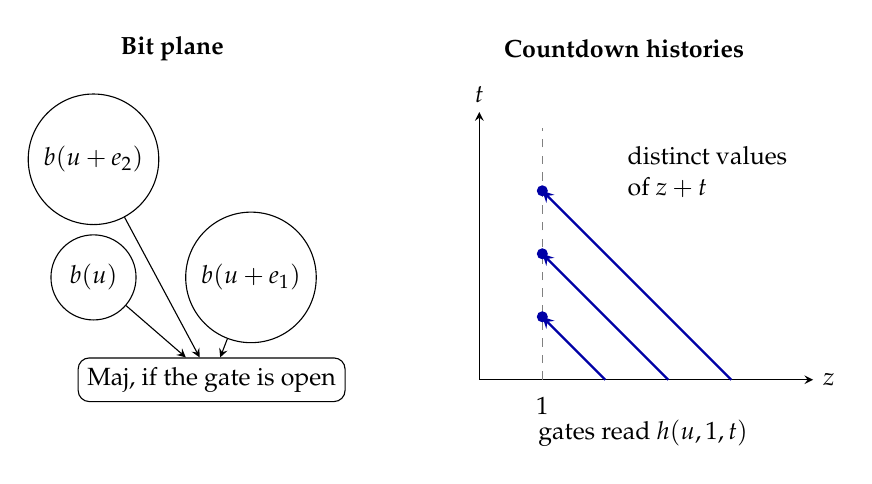
\begin{tikzpicture}[font=\small,>=stealth]
\begin{scope}[shift={(0,0)}]
\node[font=\small\bfseries] at (1.7,4.4) {Bit plane};
\node[draw,circle,inner sep=4pt] (c) at (0.7,1.5) {$b(u)$};
\node[draw,circle,inner sep=4pt] (e) at (2.7,1.5) {$b(u+e_1)$};
\node[draw,circle,inner sep=4pt] (n) at (0.7,3) {$b(u+e_2)$};
\node[draw,rounded corners] (m) at (2.2,0.2) {$\Maj$, if the gate is open};
\draw[->] (c)--(m); \draw[->] (e)--(m); \draw[->] (n)--(m);
\end{scope}
\begin{scope}[shift={(5.6,0.2)},x=0.8cm,y=0.8cm]
\node[font=\small\bfseries] at (2.3,5.25) {Countdown histories};
\draw[->] (0,0)--(5.3,0) node[right] {$z$};
\draw[->] (0,0)--(0,4.25) node[above] {$t$};
\draw[dashed,gray] (1,0)--(1,4);
\foreach \k in {1,2,3} {
\draw[blue!65!black,thick,->] (1+\k,0)--(1,\k);
\fill[blue!65!black] (1,\k) circle (2pt);
}
\node[anchor=west,align=left] at (2.2,3.3) {distinct values\\of $z+t$};
\node[anchor=north] at (1,-0.12) {$1$};
\node[align=center] at (2.6,-0.85) {gates read $h(u,1,t)$};
\end{scope}
\end{tikzpicture}
\caption{The bits use majority within one horizontal plane. The countdown read by each successive gate follows a different diagonal in the $(z,t)$ coordinates. Independent randomness on these disjoint diagonals gives independent gates.}
\label{fig:mechanism}
\end{figure}

Toom proved stability of north-east-centre majority under small errors \cite{Toom80}. We use the explicit infinite-plane estimate in G\'acs's exposition \cite{Gacs21}. The extra spatial coordinate in our construction lets the countdowns move toward a fixed data plane without reusing their random histories there; \cref{fig:mechanism} illustrates this independence.

Marsan, Sablik and T\"orm\"a already established the phenomenon of ergodicity at low and high noise, with non-ergodicity in between, for a one-dimensional cellular automaton \cite{MST26}. Their rule retains a cyclic clock in the absence of noise. Our contribution is a nilpotent rule with this behavior, and an exact reduction to a familiar two-dimensional majority process. The dependence of stationary laws on vanishing noise for nilpotent automata is also studied by Marsan and Sablik \cite{MS24}.

\begin{table}[t]
\centering\small
\begin{tabularx}{\textwidth}{@{}>{\raggedright\arraybackslash}p{0.27\textwidth} X p{0.18\textwidth}@{}}
\toprule
Result & Behavior under noise & Deterministic rule\\
\midrule
Marcovici--Sablik--Taati \cite{MST19} & Ergodicity under all sufficiently small perturbations of each fixed nilpotent rule. & Nilpotent\\[4pt]
Marsan--Sablik--T\"orm\"a \cite{MST26} & One-dimensional example with ergodicity at low and high noise, and non-ergodicity between. & Cyclic clock\\[4pt]
Douglas--Mghirbi \cite{DM26A} & Computable family on $\Z^8$ whose ergodicity at each fixed small rate is equivalent to halting. & Quorum rule\\[4pt]
This paper, Theorems~A and~D & Three-dimensional example with the same three regimes under uniform replacement noise; for each $n$, an example with $n$ separated non-ergodic windows. & Nilpotent\\[4pt]
This paper, Theorem~C & Computable family on $\Z^9$ whose ergodicity at each rate of a fixed interval is equivalent to halting. & Nilpotent\\
\bottomrule
\end{tabularx}
\caption{The nilpotent question, the earlier two-transition phenomenon and undecidable ergodicity at a fixed rate.}
\label{tab:landscape}
\end{table}

\paragraph{Reading guide.}
\Cref{sec:rule,sec:clocks} define the model and derive its independent gates. \Cref{sec:memory} imports the majority-stability estimate and proves coexistence of stationary laws. \Cref{sec:ergodicity} gives the coupling proof for the two ergodic regimes. \Cref{sec:nu-undecidable} lifts the undecidable family of \cite{DM26A} to a uniformly nilpotent family on $\Z^9$, and \cref{sec:nu-many-windows} gives, for each $n$, a nilpotent rule with $n$ separated memory windows. \Cref{sec:deterministic} proves the separated-event statement directly. The non-elementary inputs are Toom's stability theorem in the stated quantitative form and, in \cref{sec:nu-undecidable} only, the machine-to-tiling compiler, the three-token theorem and the Common local maps lemma of \cite{DM26A}.

\section{The rule and the noise}\label{sec:rule}

Write $\N=\{0,1,\ldots\}$. Fix an integer $H\geq1$ and write a site of $\Z^3$ as $(u,z)$ with $u\in\Z^2$ and $z\in\Z$. Its state belongs to
\[
\A_H=\{0,1\}\times\{0,1,\ldots,H\}.
\]
The two coordinates of a configuration are denoted by $b$ and $h$. Let $e_1,e_2$ be the positive coordinate vectors in $\Z^2$, and let $a_+=\max(a,0)$. Define the cellular automaton $F_H$ by
\begin{align}
(F_Hh)(u,z)&=(h(u,z+1)-1)_+,\label{eq:clockrule}\\
(F_Hb)(u,z)&=\ind_{\{h(u,z+1)>0\}}
 \Maj\bigl(b(u,z),b(u+e_1,z),b(u+e_2,z)\bigr).
\label{eq:bitrule}
\end{align}
The notation $F_Hh,F_Hb$ refers to the coordinates of $F_H(b,h)$. Its neighborhood consists of $0$, $(e_1,0)$, $(e_2,0)$ and $e_3=(0,0,1)$. Thus its radius in the $\ell^\infty$ metric is one.

\begin{proposition}\label{prop:nilpotent}
For every configuration, $F_H^{H+1}(b,h)$ is the uniform state $(0,0)$. The least such common exponent is $H+1$.
\end{proposition}
\begin{proof}
Induction in \eqref{eq:clockrule} gives
\[
 h_t(u,z)=(h_0(u,z+t)-t)_+.
\]
Consequently all countdowns are zero at time $H$. The next bit update is zero at every site, proving the first assertion. Starting with $b_0\equiv1$ and $h_0\equiv H$ gives $h_t\equiv H-t$ and $b_t\equiv1$ for $0\leq t\leq H$. This configuration has not reached $(0,0)$ at time $H$, proving minimality.
\end{proof}

For $0<\eps\leq1$, the noisy rule $P_{H,\eps}$ first applies $F_H$ and then, independently at each site and time, replaces the whole symbol with probability $\eps$ by a uniform element of $\A_H$. More explicitly, at times $t\geq1$ let
\[
 R_t(u,z)\sim\operatorname{Bernoulli}(\eps),\qquad
 V_t(u,z)\sim\operatorname{Bernoulli}(1/2),\qquad
 U_t(u,z)\sim\operatorname{Unif}\{0,\ldots,H\}
\]
be mutually independent over all indices. If $R_t=1$, set $(b_t,h_t)=(V_t,U_t)$ at that site; otherwise use \eqref{eq:clockrule}--\eqref{eq:bitrule} from time $t-1$. Every one-site transition probability is at least $\eps/[2(H+1)]$. The noise is therefore positive and has zero range in the terminology of \cite{MST19}.

Let $\Omega_H=\A_H^{\Z^3}$ with the product topology. A stationary law is a probability measure $\mu$ satisfying $\mu P_{H,\eps}=\mu$. We call the PCA \emph{ergodic} if it has a unique stationary law and the law from every initial configuration converges weakly to it. It is \emph{uniformly exponentially ergodic} if, for some $C,c>0$ and every finite $W\subset\Z^3$,
\begin{equation}\label{eq:uee}
 \sup_{x\in\Omega_H}\dtv\bigl((\delta_xP_{H,\eps}^t)_W,\mu_W\bigr)
 \leq C|W|e^{-ct}.
\end{equation}
All constants here may depend on $H$ and $\eps$.

The space $\Omega_H$ is compact and metrizable. Since a local observable after one update depends continuously on finitely many input symbols, the transition operator is Feller. In particular a stationary law exists: any weak limit point of the Ces\`aro averages $T^{-1}\sum_{t=0}^{T-1}\nu P_{H,\eps}^t$ is stationary. Indeed, applying $P_{H,\eps}$ to this average changes its integral against a bounded continuous observable by at most twice the supremum norm divided by $T$. We will use this elementary compactness argument for both existence and coexistence.

\section{Countdowns and independent gates}\label{sec:clocks}

Write $r=1-\eps$ in this section. At a site $(u,z)$ and time $t$, the countdown reads its past along
\begin{equation}\label{eq:characteristic}
 (u,z+a,t-a),\qquad a=0,1,\ldots,t.
\end{equation}
Along this diagonal the value of $z+t$ is constant. If the most recent replacement on it occurred $a$ steps ago, the present countdown is $(U-a)_+$. In the absence of such a replacement it is $(h_0(u,z+t)-t)_+$. Only the last $H$ update positions can affect the present value: a reset of age at least $H$ has already reached zero, as has every possible initial countdown after $H$ steps.

\begin{lemma}\label{lem:stationaryclock}
The countdown process has a stationary product law $\pi_{H,\eps}^{\otimes\Z^3}$. Its one-site marginal is the law of $(U-A)_+$, where $U$ is uniform on $\{0,\ldots,H\}$ and $A$ is independent with
\[
 \Prob(A=a)=\eps r^a,\qquad a\in\N.
\]
For every $t\geq H$ the countdown configuration has this product law from every initial configuration, and it is independent of the initial countdowns.
\end{lemma}
\begin{proof}
For one diagonal, the geometric variable $A$ records the age of the last replacement in an indefinitely extended past. At one further step its age is zero with probability $\eps$, and otherwise increases by one, which preserves this geometric law. The reset mark $U$ is independent and uniform, so the stated marginal is invariant under the countdown transition.

At a fixed time, distinct sites follow disjoint diagonals in \eqref{eq:characteristic}. Product initial countdowns and independent replacement marks therefore give independent countdowns again. This proves stationarity of the product law. At time $t\geq H$, truncating each diagonal to ages $0,\ldots,H-1$ gives exactly the same value: if there has been no replacement in these $H$ positions, the value is zero. This is the same function of the same finite set of marks for every initial countdown configuration. Disjointness of the diagonals proves the final assertions.
\end{proof}

Fix a horizontal bit plane, say $z=0$, and define its gate by
\[
 G_t(u)=\ind_{\{h_t(u,1)>0\}},\qquad t\geq0.
\]
The gate is read in the update of $b_{t+1}(u,0)$. Initialize the countdowns with the product law in \cref{lem:stationaryclock}, independently of all later marks, and initialize the bits with any deterministic configuration.

\begin{lemma}[Exact gate law]\label{lem:gates}
The variables $G_t(u)$ are independent over $(u,t)\in\Z^2\times\N$. They are independent of every replacement variable $R_s(v,0),V_s(v,0)$ in the bit plane. Their common closed-gate probability is
\begin{equation}\label{eq:q}
 q_H(\eps)=\Prob(G_t(u)=0)
 =\frac1{H+1}\sum_{j=0}^H(1-\eps)^j
 =\frac{1-(1-\eps)^{H+1}}{\eps(H+1)}.
\end{equation}
From arbitrary deterministic initial countdowns, the same assertions hold for the gates with $t\geq H$.
\end{lemma}
\begin{proof}
The primitive variables determining $G_t(u)$ lie on the diagonal
\[
 (u,1+a,t-a),\qquad 0\leq a<t,
\]
together with the initial height at $(u,1+t)$ when it is needed. A second gate either has a different $u$ or a different value of $z+t=1+t$. Its determining variables are then disjoint from the first gate's. All initial countdowns are independent, so the gates are independent. Every determining site has $z\geq1$, while the displayed bit-plane replacement variables have $z=0$. This proves their independence as well.

By \cref{lem:stationaryclock}, a gate is closed exactly when $U\leq A$. Averaging first over $U$ gives
\[
 \Prob(U\leq A)=\frac1{H+1}\sum_{j=0}^H\Prob(A\geq j)
 =\frac1{H+1}\sum_{j=0}^H r^j.
\]
Summing this geometric series proves \eqref{eq:q}. For $t\geq H$, the gate depends only on the last $H$ update positions, regardless of its initial countdown, so the preceding independence argument applies verbatim.
\end{proof}

The qualification about the initial countdowns is necessary. For example, from $h_0\equiv H$, the gates at time zero are deterministically open. The stationary initialization gives the exact law \eqref{eq:q} from the first bit update; arbitrary initialization gives it after the finite countdown transient.

\begin{proposition}[The projected majority process]\label{prop:projection}
Under the stationary countdown initialization, $B_t(u)=b_t(u,0)$ is a binary PCA with independent local random choices and update
\begin{equation}\label{eq:projection}
 B_{t+1}(u)=
 \begin{cases}
 V_{t+1}(u,0),&R_{t+1}(u,0)=1,\\
 G_t(u)\Maj(B_t(u),B_t(u+e_1),B_t(u+e_2)),&R_{t+1}(u,0)=0.
 \end{cases}
\end{equation}
The indicators
\begin{equation}\label{eq:fault}
 I_{t+1}(u)=\ind_{\{R_{t+1}(u,0)=1\ \mathrm{or}\ G_t(u)=0\}}
\end{equation}
are independent Bernoulli variables of parameter
\begin{equation}\label{eq:p}
 p_H(\eps)=\eps+(1-\eps)q_H(\eps).
\end{equation}
At every update where $I_{t+1}(u)=0$, the bit obeys north-east-centre majority exactly.
\end{proposition}
\begin{proof}
Equation \eqref{eq:projection} is the bit coordinate of the original update. Its right-hand side uses the plane's bits, its past gate variables, and its plane replacement variables. By \cref{lem:gates}, the new gates and replacements are independent of all these earlier variables and independent across $u$. This proves the PCA assertion and \eqref{eq:p}. A zero indicator in \eqref{eq:fault} means an open gate and no replacement, giving the last assertion.
\end{proof}

For clarity, the independent indicators describe opportunities for an error; a replacement may happen to write the majority value. The exact transition probability of the projected PCA is
\begin{equation}\label{eq:kernel}
 \Prob(B_{t+1}(u)=1\mid B_t)
 =\frac{\eps}{2}+(1-\eps)(1-q_H(\eps))
  \Maj(B_t(u),B_t(u+e_1),B_t(u+e_2)).
\end{equation}
The actual error probability is $\eps/2$ when the majority is zero and $\eps/2+(1-\eps)q_H(\eps)$ when it is one. Both are bounded by $p_H(\eps)$.

\section{Memory at a positive noise rate}\label{sec:memory}

We state precisely the stability estimate needed here, taken from G\'acs's exposition \cite{Gacs21} of the Berman--Simon proof \cite{BermanSimon88}. The parameter $\rho$ below bounds local update errors relative to majority, and is distinct from the replacement probability $\eps$ of our model.

\begin{theorem}[Toom stability, quantitative specialization]\label{thm:toom}
Let a binary process on $\Z^2$, started from the constant bit $a\in\{0,1\}$, be a $\rho$-perturbation of north-east-centre majority: conditional on the past, its site updates are independent and each disagrees with majority with probability at most $\rho$. If
\begin{equation}\label{eq:toomconstant}
 \rho<\tau:=\frac1{32\cdot24^8},
\end{equation}
then at every site and time its probability of disagreeing with $a$ is at most $96\rho$.
\end{theorem}

This is the infinite-plane case $m=\infty$ of the main theorem of \cite{Gacs21},\footnote{In the displayed perturbation condition of \cite{Gacs21}, the comparison with the prescribed output is printed as equality. We use the disagreement event specified by its subsequent definition of $\mathrm{Noise}$ and its proof.} specialized as follows. Take the auxiliary one-dimensional space in its Definition~1.5 to be a singleton and its transition rule to be the identity. The resulting three-dimensional rule is exactly NEC majority on the remaining two coordinates. The constant reference trajectory is $a$ at every site and time. The constants stated there are $r=24$, threshold $(32r^8)^{-1}$, and error bound $4r\rho$. Independent site updates with the displayed conditional error bound satisfy its perturbation hypothesis, including conditioning on the other simultaneous outputs. Outside \cref{sec:nu-undecidable}, this is the sole imported estimate; Toom's original theorem is \cite{Toom80}. A one-point auxiliary space is admitted by the definitions of \cite{Gacs21}; the neighbours $n\pm1$ then coincide with $n$, and its perturbation condition is read for the three-dimensional rule as in the theorem.

\begin{theorem}\label{thm:coexistence}
If $p_H(\eps)<\tau$, then $P_{H,\eps}$ has two translation-invariant stationary laws $\mu^0,\mu^1$ satisfying, at every site $v\in\Z^3$,
\begin{equation}\label{eq:phases}
 \mu^0\{b(v)=1\}\leq96p_H(\eps),\qquad
 \mu^1\{b(v)=1\}\geq1-96p_H(\eps).
\end{equation}
In particular it is non-ergodic. The condition holds for
\begin{equation}\label{eq:explicit}
 \eps_*=2^{-44},\qquad H_*=2^{88}.
\end{equation}
\end{theorem}
\begin{proof}
For $a=0,1$, let $\nu^a$ be the initial law with every bit equal to $a$ and countdowns drawn from the stationary product law. For every horizontal plane, \cref{prop:projection} is a $p_H(\eps)$-perturbation in the sense of \cref{thm:toom}. Its error probability conditional on the entire plane past is bounded by \eqref{eq:p}, and updates at the current time are conditionally independent. Thus
\[
 \Prob_{\nu^a}\{b_t(v)\ne a\}\leq96p_H(\eps)
 \qquad(v\in\Z^3,\ t\geq0).
\]
The planes need not be independent; the estimate uses their individual marginal processes.

Take a weak limit point $\mu^a$ of the Ces\`aro averages of $\nu^aP_{H,\eps}^t$. The Feller argument in \cref{sec:rule} proves stationarity. The initial laws are translation invariant and the transition commutes with translations, so the limit laws are also translation invariant. The one-site events in the preceding display are clopen cylinders, and their bounds pass to the limit, proving \eqref{eq:phases}. Since $192\tau<1$, the two bounds are disjoint and the laws differ.

For the explicit choice, \eqref{eq:q} gives
\[
 q_{H_*}(\eps_*)\leq\frac1{\eps_*(H_*+1)}<2^{-44},
 \qquad p_{H_*}(\eps_*)<2^{-43}.
\]
Also $32\cdot24^8=2^{29}3^8<2^{42}$ because $3^8=6561<8192$. Hence $2^{-43}<\tau$, as required.
\end{proof}

More generally, for every fixed $0<\eps<\tau$, a sufficiently large $H$ satisfies the hypothesis, since $q_H(\eps)\leq1/[\eps(H+1)]$. Thus the counterexample can be placed at arbitrarily small positive replacement rates by changing the automaton. For any one chosen $H$, sufficiently small noise has a different behavior, which we now prove. The existence of some $H$ and $\eps$ with two stationary laws needs only Toom's theorem \cite{Toom80} with an unspecified threshold; the constants of \cite{Gacs21} enter only in the explicit choice above.

\section{Ergodicity at small and large noise}\label{sec:ergodicity}

Couple two trajectories from arbitrary configurations by using the same replacement indicators and the same replacement symbols. Their countdowns agree everywhere by time $H$, even if no replacement occurs on a particular diagonal. Once the countdowns agree, a closed gate or a replacement makes the corresponding bit outputs agree. An open gate without a replacement can pass a disagreement only from one of the three majority parents in its own plane.

Put
\begin{equation}\label{eq:alpha}
 \alpha_H(\eps)=(1-\eps)(1-q_H(\eps)),
 \qquad \lambda_H(\eps)=3\alpha_H(\eps).
\end{equation}
The first quantity is the probability that one bit update can depend on its preceding bits.

\begin{theorem}\label{thm:contraction}
If $\lambda_H(\eps)<1$, then $P_{H,\eps}$ has a unique stationary law $\mu$ and, for every finite $W\subset\Z^3$ and $n\geq1$,
\begin{equation}\label{eq:couplingbound}
 \sup_{x\in\Omega_H}\dtv\bigl((\delta_xP_{H,\eps}^{H+n})_W,\mu_W\bigr)
 \leq |W|\lambda_H(\eps)^n.
\end{equation}
It is uniformly exponentially ergodic whenever
\begin{equation}\label{eq:regimes}
 0<\eps<\frac{2}{3H}\qquad\text{or}\qquad\frac23<\eps\leq1.
\end{equation}
\end{theorem}

The qualitative statements are known: ergodicity under small noise is \cite[Theorem~3.9]{MST19}, and ergodicity under large noise holds for every perturbed cellular automaton. The explicit ranges and the coupling bound above are what we add.
\begin{proof}
Fix a site $v=(u,z)$ and suppose its bits in the two coupled trajectories differ at time $H+n$. Trace backward from this disagreement. At each step there must be an open gate, no replacement at the output, and at least one disagreeing majority parent. Consequently there is a path of length $n$ ending at time $H$ with each backward spatial displacement in $\{0,e_1,e_2\}$, all within the plane at height $z$. Every update on this path is open and unreplaced.

There are $3^n$ possible paths. For a fixed path, the relevant gates are those with input times $H,H+1,\ldots,H+n-1$ in one fixed plane. By the last assertion of \cref{lem:gates}, they are independent with open probability $1-q_H(\eps)$. They are independent of all replacements in that plane. The probability that every update on the path is open and unreplaced is therefore exactly $\alpha_H(\eps)^n$. The union bound gives
\begin{equation}\label{eq:disagreement}
 \Prob\{b_{H+n}(v)\ne b'_{H+n}(v)\}\leq\lambda_H(\eps)^n.
\end{equation}
This argument does not require any independence between the initial disagreements and these gates: it bounds the event that a path of open, unreplaced updates exists. The countdowns already agree. Summing \eqref{eq:disagreement} over $W$ bounds the probability of any full-symbol disagreement in $W$, uniformly over the two initial configurations.

A stationary law exists by compactness. Couple a deterministic initial configuration to a sample from that law and integrate the preceding uniform bound. The coupling inequality gives \eqref{eq:couplingbound}, hence convergence to this stationary law from every start. Coupling samples from any two stationary laws gives the same bound at every $n$; sending $n$ to infinity proves uniqueness. If $0<\lambda_H(\eps)<1$, take $c=-\log\lambda_H(\eps)$ and enlarge the prefactor to cover $t\leq H$. If $\lambda_H(\eps)=0$, the trajectories agree after at most $H+1$ steps, which also implies \eqref{eq:uee}.

It remains to check \eqref{eq:regimes}. Bernoulli's inequality in \eqref{eq:q} yields
\[
 q_H(\eps)\geq\frac1{H+1}\sum_{j=0}^H(1-j\eps)
 =1-\frac{H\eps}{2}.
\]
Thus $\lambda_H(\eps)\leq3H\eps/2<1$ in the small-noise range. For large noise, $\lambda_H(\eps)\leq3(1-\eps)<1$.
\end{proof}

\begin{corollary}[Re-entrance]\label{cor:reentrance}
For the single rule $F_{H_*}$ in \eqref{eq:explicit}, there is an open interval of positive noise rates containing $\eps_*$ on which the PCA is non-ergodic. It is uniformly exponentially ergodic at every rate in $(0,2/(3H_*))$ and $(2/3,1]$.
\end{corollary}
\begin{proof}
For fixed $H_*$ the expression $p_{H_*}(\eps)$ is continuous on $(0,1]$. The strict inequality proved in \cref{thm:coexistence} persists in a neighborhood of $\eps_*$. The two ergodic ranges follow from \cref{thm:contraction}. They lie on either side of $\eps_*$ because $2/(3\cdot2^{88})<2^{-44}<2/3$.
\end{proof}

These sufficient conditions establish ergodicity, non-ergodicity and ergodicity in that order as the noise rate increases. They do not locate the boundaries between the regimes. The exact contraction condition $3(1-\eps)(1-q_H(\eps))<1$ can also apply beyond the two intervals in \eqref{eq:regimes}.

\section{Nilpotency and undecidable noisy ergodicity}\label{sec:nu-undecidable}

The countdown mechanism transfers an undecidable noisy-ergodicity classification to a family consisting entirely of nilpotent automata. The dimension is nine and the countdown bound is the same for every member.

\paragraph{Published input and credit.}
We use our paper \cite{DM26A}, hereafter paper~A, specifically \cite[Corollary~9.21 and Lemma~8.11]{DM26A}; the latter is its Common local maps lemma. The machine-to-Wang-set compiler and the quorum and contour estimates are imported from that paper. So is its three-token theorem, whose proof includes one finite lemma that is checked by computer there \cite[Lemma~9.12]{DM26A}. The lift, its burn-in justification, the endpoint bounds and the multiple-window construction are proved here. The countdown mechanism and diagonal independence are those of the preceding sections. We assume no independence between fuel tracks or between different horizontal planes.

Set
\begin{equation}\label{eq:nu-constants}
 \eps_0=490000^{-99},\quad H_0=2\cdot490000^{198},\quad
 I_0=[\eps_0/2,\eps_0],\quad \eps_\dagger=\eps_0/2.
\end{equation}
The rate $\eps_0$ is the rate of \cite[Corollary~9.21]{DM26A}.

\begin{theorem}[Nilpotency and undecidability]\label{thm:nu-main}
There is a total computable map $M\mapsto N_M$ from Turing machines to finite-alphabet, radius-one cellular automata on $\Z^9$ such that:
\begin{enumerate}[label=\textup{(\roman*)}]
\item every $N_M$ maps every configuration to the same uniform fixed configuration after $H_0+1$ deterministic updates;
\item for every $\eps\in I_0$, uniform replacement on the entire alphabet of $N_M$ at rate $\eps$ is ergodic if and only if $M$ halts;
\item for every $M$, this perturbation is uniformly exponentially ergodic whenever
\[
 0<\eps<\frac{2}{63H_0}\quad\text{or}\quad\frac{62}{63}<\eps\le1.
\]
\end{enumerate}
The alphabet of $N_M$ depends on $M$; the rate interval, radius, dimension and nilpotency time do not. If $M$ does not halt and $\eps\in I_0$, there are at least two translation-invariant stationary laws. Thus ergodicity at the single rational rate $\eps_\dagger$ is undecidable even within this uniformly nilpotent family.
\end{theorem}

\subsection{The exact imported interface}

Paper~A gives a total computable map $M\mapsto R_M$ from Turing machines to finite Wang sets \cite[Definition~6.17]{DM26A}. Let $T_{R_M}$ be the set of legal $3\times3$ blocks of $R_M$ and put
\[
 \mathcal B_M=(T_{R_M}\times\{0,1\})\cup\{\bot\}.
\]
The symbols other than $\bot$ are \emph{live}. The planar checker keeps the symbol at a site precisely when that symbol is live and its eight Moore neighbors are live and compatible with it, that is, they carry the same checker bit and their blocks agree with its block where they overlap; otherwise it returns $\bot$ \cite[Definition~2.5]{DM26A}. In $\Z^2\times\Z^6$, perform this checker in each $\Z^2$ plane. The quorum rule $F_M=F^{[6]}_{R_M}$ returns a live symbol if at least six of the seven checked readings at transverse displacements $0,e_1,\ldots,e_6$ equal it, and returns $\bot$ otherwise \cite[Definition~2.7]{DM26A}. Its neighborhood is
\begin{equation}\label{eq:nu-neighborhood}
 \mathcal N=\{-1,0,1\}^2\times\{0,e_1,\ldots,e_6\},
 \qquad |\mathcal N|=63.
\end{equation}
All finite tables are enumerable from $M$. If $M$ does not halt, $R_M$ tiles \cite[Proposition~6.18]{DM26A}; a \emph{cloned tiling} is then the configuration that carries the blocks of one tiling, with checker bit $0$, identically on every plane \cite[Definition~4.1]{DM26A}. If $M$ halts, $R_M$ is refuted by three tokens \cite[Theorem~9.1]{DM26A}, with some finite refutation time $\tau_M$.

A random field of local maps is $\gamma$-bounded \cite[Definition~8.10]{DM26A} if the maps agree with $F_M$ away from designated faults and, for every finite set $S$ of logical spacetime points of positive time,
\begin{equation}\label{eq:nu-joint}
 \Prob(\text{every point of }S\text{ is faulty})\le\gamma^{|S|}.
\end{equation}
Logical time is counted from the start of the field: from physical time $0$, or from physical time $H_0$ after the burn-in below. The same maps drive both starts. Paper~A's Common local maps lemma \cite[Lemma~8.11]{DM26A} says the following. For $0<\gamma\le2\eps_0$, write
\[
 D_0=350,\qquad
 \beta=2D_0^2\gamma^{1/99},\qquad
 \ell=2D_0^2\gamma^{1/49},
\]
with the constants of \cite[Corollary~9.21]{DM26A}. If $M$ halts, the common-map coupling from any two deterministic starts obeys
\begin{equation}\label{eq:nu-import-forget}
 \Prob(X_s(v)\ne Y_s(v))
 \le \frac{2\gamma^{-\tau_M/99}\beta^s}{1-\beta}.
\end{equation}
If $M$ does not halt, a run from any cloned tiling $\xi$ differs from $\xi$ at a given site with probability at most $\gamma(1+2\ell/(1-\ell))<1.01\gamma$; a run from bottom is live there with probability less than $1.01\gamma$, at every time. These conclusions allow arbitrary faulty maps satisfying \eqref{eq:nu-joint}. We will have iid faults and constant maps at faults.

For completeness, the numerical margins are explicit:
\[
 \beta\le2^{1/99}/2<13/25,\qquad
 \ell\le\frac{2^{1/49}}{8\cdot350^2}<\frac1{490000}.
\]
Indeed $(26/25)^{99}\ge1+99/25>2$; also $99/49>2$ and $2^{1/49}<2$. Thus $1+2\ell/(1-\ell)<1.01$. Since $\gamma<1/1000$, the gap $1-2.02\gamma$ is positive. Here $\tau_M$ is the time coordinate of any finite refutation witness. It is unnecessary for constructing $N_M$; no total computable bound on this convergence parameter is asserted.

\subsection{A general countdown lift}

Let $F$ be any cellular automaton on $\mathcal B^{\Z^d}$ whose local rule $f$ reads $m\ge1$ inputs, and choose $\bot\in\mathcal B$. For an integer $K\ge1$, its lift on $\Z^d\times\Z$ has alphabet $\mathcal B\times\{0,\ldots,K\}$ and rule
\begin{align}
 h'(v,z)&=(h(v,z+1)-1)_+,\label{eq:nu-lift-h}\\
 b'(v,z)&=
 \begin{cases}
 F(b(\cdot,z))(v),&h(v,z+1)>0,\\
 \bot,&h(v,z+1)=0 .
 \end{cases}\label{eq:nu-lift-b}
\end{align}
The data symbol $b$ need not be binary. Quiescence of $\bot$ for $F$ is unnecessary.

\begin{lemma}[Exact slice law and burn-in]\label{lem:nu-slice}
The lift is nilpotent by time $K+1$. Under uniform replacement of its entire symbol at rate $0<\eps\le1$, put
\[
 q_K(\eps)=\frac1{K+1}\sum_{j=0}^K(1-\eps)^j
          =\frac{1-(1-\eps)^{K+1}}{\eps(K+1)},\qquad
 p_K(\eps)=\eps+(1-\eps)q_K(\eps).
\]
For any fixed height $z$, from time $K$ its data evolve by independent local maps with iid fault indicators of parameter $p_K(\eps)$. At a nonfault point the map is $F$. The entire future slice map field is independent of the data slice at time $K$, and of the pair of data slices there in a common-noise coupling. With stationary product fuel initialization, independent of the initial data and all subsequent noise, the exact slice law holds from time zero. Its kernel is
\begin{equation}\label{eq:nu-Q}
 Q(s\mid y)=(1-\eps)(1-q_K(\eps))\ind_{\{s=f(y)\}}
 +(1-\eps)q_K(\eps)\ind_{\{s=\bot\}}+\frac{\eps}{|\mathcal B|},
\end{equation}
where $y\in\mathcal B^m$ is the tuple of inputs read by the local rule $f$ of $F$.
\end{lemma}

\begin{proof}
Noiselessly, $h_t(v,z)=(h_0(v,z+t)-t)_+$. All fuels vanish at $K$ and the next data update is bottom. The resulting uniform state is fixed because its gates are closed.

At each physical spacetime point use independent variables: a Bernoulli coin $R$ with parameter $\eps$, a uniform fuel mark $U\in\{0,\ldots,K\}$, and a uniform data mark $V\in\mathcal B$. On $R=1$ write $(V,U)$; otherwise apply the deterministic rule. The two coordinates share $R$, exactly as uniform replacement requires.

The history of the gate reading $h_t(v,z+1)$ lies on
\[
 (v,z+1+a,t-a),\quad a\ge0,
\]
with invariant $(v,z+1+t)$. A reset of age $a$ supplies $(U-a)_+$. Resets of age at least $K$, and all initial fuels after $K$ updates, supply zero. Thus all dependence on initial fuel vanishes by time $K$. The stationary marginal is $(U-A)_+$ where $\Prob(A=a)=\eps(1-\eps)^a$ independently of $U$. Independent copies across sites are stationary, since distinct sites at one time use disjoint characteristics. Averaging over $U$ gives
\[
 \Prob((U-A)_+=0)
 =\frac1{K+1}\sum_{j=0}^K\Prob(A\ge j)=q_K(\eps).
\]

At the fixed data height $z$, different logical $(v,t)$ gates have different invariants or different $v$, hence disjoint histories. All determining sites are strictly above $z$, disjoint from every replacement primitive in the data slice. The gates are therefore independent over logical spacetime and independent of in-slice replacements. With stationary product fuels this holds from time zero. For arbitrary initial fuels, gates of input times $t\ge K$ have forgotten the initial state and have the same iid law. The union of a closed gate and an in-slice replacement is an iid fault with parameter $p_K(\eps)$. A replacement writes $V$; a closed gate without replacement writes bottom; all other points apply $F$. This proves \eqref{eq:nu-Q}.

It remains to justify restarting at a random time-$K$ slice. Its history through $K$ uses only initial data and fuels, in-slice replacements through $K$, and gates of input times $0,\ldots,K-1$, whose invariants are $z+1,\ldots,z+K$. Future gates have invariants $z+K+1,z+K+2,\ldots$, use only noise, and lie strictly above the plane. Future in-slice replacements are fresh. These sets of primitives are disjoint, proving independence from the pair of time-$K$ data slices. The argument also permits random initial configurations independent of the noise. Independence from other slices' past is not asserted or required.
\end{proof}

\begin{lemma}[Endpoint coupling]\label{lem:nu-endpoints}
Put $\lambda_K(\eps)=m(1-\eps)(1-q_K(\eps))$. If $\lambda_K(\eps)<1$, the lift has a unique stationary law $\mu$ and for every finite physical window $W$ and integer $s\ge1$,
\begin{equation}\label{eq:nu-endpoint-tv}
 \sup_x\dtv((\delta_xP^{K+s})_W,\mu_W)
 \le |W|\lambda_K(\eps)^s.
\end{equation}
This holds in particular for $0<\eps<2/(mK)$ or $1-1/m<\eps\le1$.
\end{lemma}

\begin{proof}
Use common physical noise for two arbitrary starts. Their fuels agree everywhere by $K$. Any later data discrepancy needs an open unreplaced update and a discrepant parent among the $m$ inputs in its slice. Trace $s$ steps backward from a discrepancy at $K+s$. There are at most $m^s$ possible paths. For any fixed path its distinct spacetime gates and replacement coins are independent, so all updates are open and unreplaced with probability $[(1-\eps)(1-q_K(\eps))]^s$. The union bound gives $\lambda_K(\eps)^s$. This bounds existence of a transmitting path and does not condition on the data at $K$.

Sum over $W$ to bound full-symbol discrepancies. A stationary law exists by compactness and Feller continuity. Coupling to it proves \eqref{eq:nu-endpoint-tv}; coupling two stationary laws proves uniqueness by letting $s\to\infty$. For $0<\lambda_K<1$, one may take exponential constants $c=-\log\lambda_K$ and $C=\lambda_K^{-K}$ for all times. If $\lambda_K=0$, there is finite-time coupling.

Finally, $(1-\eps)^j\ge1-j\eps$ implies $1-q_K(\eps)\le\eps K/2$. Hence $\lambda_K\le m\eps K/2$ and $\lambda_K\le m(1-\eps)$, giving both intervals. At $\eps=1$ one update is iid uniform.
\end{proof}

\begin{proof}[Proof of \cref{thm:nu-main}]
Use $F=F_M$, $d=8$, $K=H_0$ in the lift. Its alphabet is $\mathcal D_M=\mathcal B_M\times\{0,\ldots,H_0\}$. Its neighborhood consists of $\mathcal N\times\{0\}$ and the positive ninth-coordinate neighbor: $64$ sites, of radius one. Its table is total computable from $M$. The slice lemma gives nilpotency by $H_0+1$, uniformly in $M$.

For $\eps\in I_0$,
\[
 q_{H_0}(\eps)\le\frac1{\eps(H_0+1)}
 \le\frac2{\eps_0(H_0+1)}<\eps_0,\qquad p_{H_0}(\eps)<2\eps_0.
\]
Fix $\gamma=2\eps_0$. For every finite set $S$ of logical spacetime points of positive time within one slice, the exact identity
\[
 \Prob(S\text{ all faulty})=p_{H_0}(\eps)^{|S|}\le\gamma^{|S|}
\]
verifies the full joint hypothesis of paper~A.

If $M$ halts, couple two complete initial configurations using common physical noise. Fuels have coupled by $H_0$. By the burn-in independence in the slice lemma, condition on the pair of data slices at $H_0$ and apply \eqref{eq:nu-import-forget}. (Alternatively, the certificate event in the proof of \cite[Lemma~8.11(ii)]{DM26A} depends on the fault field alone and contains the disagreement for every pair of starts, so no conditioning is needed.) For every finite physical window $W$ and $s\ge1$,
\begin{equation}\label{eq:nu-global-forget}
 \sup_{x,y}\Prob(X_{H_0+s}|_W\ne Y_{H_0+s}|_W)
 \le\frac{2|W|\gamma^{-\tau_M/99}\beta^s}{1-\beta},
 \qquad \beta=2^{1/99}/2<13/25 .
\end{equation}
This union bound uses one common full-process coupling; correlations between heights cause no difficulty. Coupling to a stationary law gives attraction and uniqueness. Uniform exponential constants, including the burn-in, are $c=-\log\beta$ and $C=2\gamma^{-\tau_M/99}\beta^{-H_0}/(1-\beta)$. Every convergence constant is explicit for a finite refutation witness; that witness is unnecessary in the construction.

If $M$ does not halt, clone a tiling configuration through all heights, and independently use stationary product fuels. For the other initial law use all-bottom data and stationary fuels. Every slice has its iid map law from the first update. The imported memory estimates give, at every physical site and time,
\[
 \Prob_{\rm live}(b_t\ne\bot)\ge1-1.01\gamma,\qquad
 \Prob_{\rm bottom}(b_t\ne\bot)\le1.01\gamma.
\]
Take simultaneous subsequential Ces\`aro limits of these two full-process laws. Both limits are stationary by Feller continuity. The live-symbol cylinder is clopen, so the positive probability gap passes to the limits. The stationary laws are distinct. For translation invariance, first average a tiling over expanding planar boxes and take a limit supported on tilings. The boundary-to-volume estimate makes this law shift invariant. Clone it through all transverse coordinates and heights. Both initial full laws, and thus their Ces\`aro limits, are then translation invariant; all estimates survive integration over tilings.

Finally the endpoint lemma with $m=63$ gives the claimed explicit small- and large-noise ranges.
\end{proof}

\paragraph{A second imported interface.}
The exact projected law \eqref{eq:nu-Q} is $F$ followed by replacement at rate $p_K(\eps)$ with law
\[
 \nu=\frac{\eps\,\operatorname{Unif}(\mathcal B)
 +(1-\eps)q_K(\eps)\delta_\bot}{p_K(\eps)}.
\]
Thus the proof of paper~A's other-replacement-law corollary \cite[Corollary~8.6 and Remark~9.22]{DM26A}, which gives the per-site common-noise coupling bound for $\nu$-replacement with the same constants, can replace \eqref{eq:nu-import-forget}; it is applied in each slice after burn-in and summed over a window exactly as above, and its part~(ii) replaces the memory estimates. Take $K=8\cdot490000^{198}$ and $\eps\in[\eps_0/4,\eps_0/2]$. Then $q_K(\eps)<\eps_0/2$ and $p_K(\eps)<\eps_0$, within its original threshold. This route does not require the extension to arbitrary faulty maps. Physical noise in either construction remains exactly uniform replacement of the entire symbol.

\section{Arbitrarily many separated memory windows}\label{sec:nu-many-windows}

\begin{theorem}[Any prescribed number of windows]\label{thm:nu-windows}
For each integer $n\ge1$ there is a radius-one nilpotent cellular automaton on $\Z^3$ with $n$ disjoint open intervals of replacement rates having two translation-invariant stationary laws, separated in order by $n-1$ open intervals of uniform exponential ergodicity. It is also uniformly exponentially ergodic at all sufficiently small and all sufficiently large positive rates. All capacities and intervals are explicit.
\end{theorem}

\begin{proof}
Set
\[
 L=2^{50}(n+1),\quad
 H_i=L^{2(2n-i+1)}\ (1\le i\le2n),\quad K=H_1=L^{4n}.
\]
Use alphabet $\{0,1\}\times\prod_{i=1}^{2n}\{0,\ldots,H_i\}$. Let $\mathcal G(h)$ be the indicator that for some $j$, $h_{2j-1}>0$ and $h_{2j}=0$. The rule is
\begin{align*}
 h_i'(u,z)&=(h_i(u,z+1)-1)_+,\\
 b'(u,z)&=\mathcal G(h(u,z+1))
     \Maj(b(u,z),b(u+e_1,z),b(u+e_2,z)).
\end{align*}
All fuels vanish at $K$, and all bits at $K+1$. This is the least nilpotency exponent: initial bits one, $h_1=K$ and all other fuels zero keep all bits one through time $K$.

Under uniform replacement of the whole symbol, the reset coin is shared; conditional on replacement its bit and fuel marks are independent uniforms. The stationary joint fuel vector at a site is $((U_i-A)_+)_{i=1}^{2n}$, where the $U_i$ are independent uniforms and $\Prob(A=a)=\eps(1-\eps)^a$ is one common age. The tracks are generally dependent. Independent copies of this vector across sites are stationary; all initial fuels are forgotten by $K$. The slice lemma's disjoint-characteristic proof applies to this vector. Therefore, within each bit slice, gates are iid over spacetime and independent of in-plane replacements, from stationary initialization or after burn-in $K$. Writing $g(\eps)=\Prob(\mathcal G=1)$, the projected kernel is
\[
 \Prob(B_{t+1}(u)=1\mid B_t)
 =\eps/2+(1-\eps)g(\eps)
       \Maj(B_t(u),B_t(u+e_1),B_t(u+e_2)).
\]
Its iid majority-fault opportunities have probability $p(\eps)=\eps+(1-\eps)(1-g(\eps))$. For any track of capacity $\kappa$ the preceding calculation gives
\begin{equation}\label{eq:nu-track}
 \Prob(h=0)\le\frac1{\eps(\kappa+1)},\qquad
 \Prob(h>0)\le\eps\kappa/2.
\end{equation}

Define
\[
 w_j=L^{-[4(n-j)+3]},\quad I_j=(w_j/2,2w_j)
 \qquad(1\le j\le n).
\]
Pair $j$ has long capacity $L^{4(n-j)+4}$ and short capacity $L^{4(n-j)+2}$. For $\eps\in I_j$, a union bound using \eqref{eq:nu-track} yields
\[
 1-g(\eps)\le\Prob(h_{2j-1}=0)+\Prob(h_{2j}>0)<2/L+1/L=3/L.
\]
Also $\eps<2/L^3\le1/L$, so $p(\eps)<4/L$. Since $L\ge2^{51}$,
\[
 p(\eps)<2^{-49}<2^{-42}<\tau,
\]
with $\tau$ the threshold in \eqref{eq:toomconstant}. Indeed $32\cdot24^8=2^{29}3^8<2^{42}$. From constant bits $a=0,1$ and stationary joint-product fuel, the exact projected PCA satisfies \cref{thm:toom} with its perturbation parameter equal to $p(\eps)$. Consequently $\Prob(b_t\ne a)\le96p(\eps)$ at every physical site and time. Ces\`aro limits give two translation-invariant stationary laws with separated bit marginals, since $192\tau<1$. Every $I_j$ is therefore nonergodic.

For $1\le j<n$ set
\[
 s_j=L^{-[4(n-j)+1]},\qquad J_j=(s_j/2,2s_j).
\]
At $\eps\in J_j$, a pair $\ell\le j$ can open only if its short track is zero. Its short capacity is at least $L^{4(n-j)+2}$, so its opening probability is less than $2/L$. A pair $\ell>j$ can open only if its long track is positive. Its long capacity is at most $L^{4(n-j)}$, so its opening probability is less than $1/L$. Thus
\[
 g(\eps)<(n+j)/L\le2n/L,\qquad
 \lambda(\eps):=3(1-\eps)g(\eps)<6n/L<1 .
\]
All these estimates use union bounds, not independent tracks. Common-noise coupling erases initial fuels by $K$; each later bit discrepancy needs an open unreplaced majority-parent path. The endpoint lemma's proof, with three parents and opening probability $g(\eps)$, gives
\[
 \sup_x\dtv((\delta_xP^{K+t})_W,\mu_W)
 \le |W|\lambda(\eps)^t.
\]
Hence every $J_j$ is uniformly exponentially ergodic. This is a full-process estimate and requires no independence between heights.

The intervals lie in $(0,1)$, and $s_j/w_j=w_{j+1}/s_j=L^2>4$ gives their strict order
\[
 I_1<J_1<I_2<\cdots<J_{n-1}<I_n .
\]
For $n=1$ there are no separators. Finally $g(\eps)\le\sum_j\Prob(h_{2j-1}>0)\le\eps nK/2$. The same path coupling gives endpoint ergodicity for $0<\eps<1/(3nK)$ and $2/3<\eps\le1$. These ranges lie below $I_1$ and above $I_n$, respectively.
\end{proof}

\begin{remark}[Infinite windows remain open]\label{rem:nu-infinite}
This theorem supplies a different finite-alphabet rule for each $n$. It does not give one rule with infinitely many alternating windows. There is a precise limitation of these certificates for finite tracks. Conditioning on the common reset age $a$, independent reset marks give
\[
 G(a)=1-\prod_{j=1}^n\left[
 1-\frac{(H_{2j-1}-a)_+}{H_{2j-1}+1}
       \frac{\min(a,H_{2j})+1}{H_{2j}+1}
 \right].
\]
As $G(a)=0$ for $a\ge K$,
\[
 g(\eps)=\sum_{a=0}^{K-1}\eps(1-\eps)^aG(a)
\]
is a rational-coefficient polynomial. So are $p(\eps)=1-(1-\eps)g(\eps)$ and $\lambda(\eps)=3(1-\eps)g(\eps)$. Their strict certificate sets $p<\tau$ and $\lambda<1$ have finitely many components: a nonzero boundary polynomial has finitely many roots; an identically zero one gives no strict certificate on its boundary. This is a finiteness statement about these two sufficient certificates, not about the actual phase diagram. A single nilpotent finite-alphabet automaton with infinitely many alternating nonergodic windows remains open here.
\end{remark}

\section{Separated deterministic replacement events}\label{sec:deterministic}

A replacement event is a point $(u,z,s)\in\Z^2\times\Z\times\N_{\geq1}$ at which, after the deterministic update into time $s$, a prescribed symbol overwrites the output. All other updates follow $F_H$. Distances between events are measured in all four coordinates using $\ell^\infty$. In particular, separation in the $z$ coordinate suffices even when events have the same time.

\begin{theorem}\label{thm:separation}
Given $d\geq0$, choose an integer $m>d$ and let $H=m^4$. There is a set $\mathcal E$ of replacement events at pairwise $\ell^\infty$ distance at least $m$ such that every event writes $(0,H)$, and the two initial configurations
\[
 (b_0,h_0)\equiv(0,H),\qquad (b'_0,h'_0)\equiv(1,H)
\]
produce $b_t(u,0)=0$ and $b'_t(u,0)=1$ for every $u\in\Z^2$ and $t\geq0$ under these common events. The underlying rule is nilpotent of exponent $H+1$.
\end{theorem}
\begin{proof}
For $u=(x,y)$ and $t\geq H$, let $[x]_m,[y]_m,[t]_m\in\{0,\ldots,m-1\}$ be their residues, and set
\begin{equation}\label{eq:color}
 c(u,t)=[x]_m+m[y]_m+m^2[t]_m,
 \qquad a(u,t)=m\,c(u,t).
\end{equation}
The age satisfies $0\leq a(u,t)\leq m^4-m=H-m$. Place one event for each such pair $(u,t)$ at
\begin{equation}\label{eq:event}
 E(u,t)=\bigl(u,1+a(u,t),t-a(u,t)\bigr),
\end{equation}
and let every event write $(0,H)$. Its time is at least $m\geq1$, and its height coordinate is positive, so these are valid events and none belongs to the bit plane $z=0$.

We first check separation. If two ages in \eqref{eq:event} differ, their $z$ coordinates differ by a nonzero multiple of $m$, hence by at least $m$. If the ages agree, the residue triples in \eqref{eq:color} agree. Distinct pairs $(u,t)$ then differ in at least one of $x,y,t$ by a nonzero multiple of $m$. Equal ages preserve that difference in the corresponding event coordinates $x,y,s=t-a$. The events are therefore distinct and at pairwise distance at least $m>d$.

We next check that the gates into $z=0$ are always open. With initial countdowns equal to $H$, and all subsequent resets equal to $H$, monotonicity of the decrement map gives
\[
 h_t(u,1)\geq(H-t)_+.
\]
This is positive for $0\leq t<H$. For $t\geq H$, the event $E(u,t)$ puts a countdown $H$ on the backward diagonal of $(u,1,t)$, at age $a=a(u,t)<H$. Propagating this value forward along that diagonal gives a countdown at least $H-a\geq m>0$ at $(u,1,t)$. Any intervening reset sets the countdown to $H$ and can only increase this lower bound. Hence every gate into the bit plane is open at every time.

The bits at $z=0$ are never replaced and read bits only in that plane. They consequently follow exact NEC majority forever. The two constant initial bit planes remain respectively zero and one, proving the claimed discrepancy. Nilpotency of the rule without replacements is \cref{prop:nilpotent}.
\end{proof}

The separation parameter is fixed before the automaton is chosen. Thus the theorem provides arbitrarily well separated renewal events across the family of nilpotent rules. Their positions in the extra spatial coordinate keep the renewals separated while feeding every gate of the same bit plane.

\section{How this work was done}

\paragraph{AI note.}
The authors chose the question, directed the work and judged every result. AI models from two developers assisted. For version~1.0.0, OpenAI's GPT-6 proposed the countdown construction, and Anthropic's Claude Opus~5.5 checked it by hand. OpenAI's GPT-6.1~Sol, through Codex, searched the literature, wrote the proofs and prepared the manuscript. Anthropic's Claude Fable~5.2 read the manuscript refutation-first, in two rounds, before release, and its findings were fixed.

Version~1.1.0 adds \cref{sec:nu-undecidable,sec:nu-many-windows}. OpenAI's GPT-6.1~Sol derived them, and separate agents of the same model family audited the lift, the imported interface and the window construction refutation-first. Anthropic's Claude Opus~5.5 then checked both sections refutation-first, as a review from the other developer. It found no error in the mathematics and suggested presentational changes, which this version makes; a separate run of Claude Opus~5.5 integrated the sections and those changes into the manuscript.

Models are not listed as authors; the authors take responsibility for every claim. The proofs of the countdown reduction, coupling bound, separated-event construction, countdown lift and window construction are given in full, and none of them uses a computation. The majority-stability estimate is imported from \cite{Gacs21}; its specialization and constants are stated in \cref{thm:toom}. \Cref{sec:nu-undecidable} also imports the machine-to-tiling compiler, the three-token theorem and the Common local maps lemma of \cite{DM26A}; the proof of the three-token theorem there includes one finite lemma that is checked by computer \cite[Lemma~9.12]{DM26A}.

\begin{thebibliography}{9}\raggedright
\bibitem{Gacs21}
P. G\'acs, \emph{A new version of Toom's proof}, 2021.
\href{https://arxiv.org/abs/2105.05968v1}{arXiv:2105.05968v1}.

\bibitem{MST19}
I. Marcovici, M. Sablik and S. Taati,
\emph{Ergodicity of some classes of cellular automata subject to noise},
Electronic Journal of Probability \textbf{24} (2019), paper 41, 1--44.
\href{https://doi.org/10.1214/19-EJP297}{doi:10.1214/19-EJP297}.

\bibitem{MS24}
H. Marsan and M. Sablik, \emph{Strong stochastic stability of cellular automata}, 2024.
\href{https://arxiv.org/abs/2403.19932}{arXiv:2403.19932}.

\bibitem{MST26}
H. Marsan, M. Sablik and I. T\"orm\"a,
\emph{A perturbed cellular automaton with two phase transitions for the ergodicity},
Journal of Statistical Physics \textbf{193} (2026), article 6.
\href{https://doi.org/10.1007/s10955-025-03564-0}{doi:10.1007/s10955-025-03564-0}.

\bibitem{BermanSimon88}
P. Berman and J. Simon, \emph{Investigations of fault-tolerant networks of computers},
in \emph{Proceedings of the 20th Annual ACM Symposium on Theory of Computing}, 1988, 66--77.

\bibitem{Toom80}
A. L. Toom, \emph{Stable and attractive trajectories in multicomponent systems},
in \emph{Multicomponent Random Systems}, R. L. Dobrushin and Ya. G. Sinai (eds.),
Adv. Probab. Related Topics \textbf{6}, Marcel Dekker, New York, 1980, 549--575.

\bibitem{DM26A}
S. Douglas and N. Mghirbi, \emph{Forgetting under noise is undecidable:
ergodicity of positive-rate cellular automata at a fixed noise rate},
version 1.3.0, 2026.
\href{https://doi.org/10.5281/zenodo.24115709}{doi:10.5281/zenodo.24115709}.
\end{thebibliography}
\end{document}
